\documentclass[a4paper,10pt]{article}
\usepackage[utf8]{inputenc}
\usepackage{xcolor}
\usepackage{graphicx}
\usepackage{float}
\usepackage{listings}   %for code
\usepackage[font={small,bf}]{caption}
\usepackage{authblk}    %for affil in title page
\usepackage[colorlinks=true,linkcolor=blue,citecolor=red, urlcolor=red]{hyperref}
\usepackage{color}
\usepackage[english]{babel}
\usepackage{amsmath}

\definecolor{codegreen}{rgb}{0,0.6,0}
\definecolor{codegray}{rgb}{0.5,0.5,0.5}
\definecolor{codepurple}{rgb}{0.58,0,0.82}
\definecolor{backcolour}{rgb}{0.97,0.97,0.97}

\lstdefinestyle{mystyle}{
    backgroundcolor=\color{backcolour},
    commentstyle=\color{codegreen},
    keywordstyle=\color{blue},
    numberstyle=\tiny\color{codegray},
    stringstyle=\color{codepurple},
    basicstyle=\ttfamily\footnotesize,
    breakatwhitespace=false,
    breaklines=true,
    captionpos=b,
    keepspaces=true,
    numbers=left,
    numbersep=5pt,
    showspaces=false,
    showstringspaces=false,
    showtabs=false,
    tabsize=2,
    morecomment=[l][\color{codegreen}]{\#}
}

\lstset{style=mystyle}

\begin{document}

\begin{titlepage} % Suppresses displaying the page number on the title page and the subsequent page counts as page 1
	
	\raggedleft % Right align the title page
	
	\rule{1pt}{\textheight} % Vertical line
	\hspace{0.02\textwidth} % Whitespace between the vertical line and title page text
	\parbox[b]{0.75\textwidth}{ % Paragraph box for holding the title page text, adjust the width to move the title page left or right on the page
		
		{\Huge\bfseries TDT4287}\\[2\baselineskip] % Title
		{\large\textit{Preprocessor for high throughput sequencing reads}}\\[4\baselineskip] % Subtitle or further description
		{\Large\textsc{roc salvador\\marc falcón}} % Author names, lower case for consistent small caps
		
		\vspace{0.5\textheight} % Whitespace between the title block and the publisher
		
		{\noindent \today}\\[\baselineskip] % Date
	}

\end{titlepage}


\tableofcontents

\newpage

\section{Task 1} \label{task1}

\paragraph{} The first task consists on developing an algorithm that identifies all the sequences in S that contain suffixes that perfectly.
match a prefix of the given adapter sequence.

\subsection{Trie}

\paragraph{} For Task \ref{task1} and Task \ref{task2} we used a trie as a data structure to store the prefixes of the adapter sequence.
A trie is structured as a tree, where each node contains a letter and each node has childs that represent the next letters of the words stored in the trie. 
You can see an example in the following picture \ref{trie-example}.

\begin{figure}[H]
    \centering
    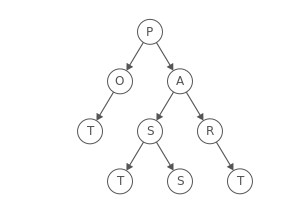
\includegraphics[width=7cm, height=5cm]{images/trie.png}
    \caption{Trie for "part", "pot", "past" and "pass"}
    \label{trie-example}
\end{figure}

\begin{lstlisting}[language=c++, caption=Our trie implementation]
class Trie {
    struct Node {
        // Childs of the current node,
        // in our case can only be 4: 'A', 'C, 'G' and 'T'
        // A child is NULL if it does not exist
        Node*[] childs = Node*[4];
        // True if a node is a valid end of a word, false otherwise
        bool isWordEnd;         
        // True if a node is a leaf of the tree, false otherwise
        bool isLeaf;            
    };

    Node* root;
};
\end{lstlisting}


\subsection{Perfect suffix-prefix match}

To solve the prefix-suffix problem we use the algorithm presented next we have to create a trie with all the suffixes of the reversed adapter sequence and then the sequences have to be reversed when searched.

Example:
$$ A = ACGACG $$
$$ reversedA = GCAGCA $$
$$ S = TACG $$
$$ reversedS = GCAT $$

$$root-G-C-A(word end)-G-C-A(wordend)$$
$$root-C-A(wordend)-G-C-A(wordend)$$
$$root-A(wordend)-G-C-A(wordend)$$
If we search in the trie the $reversedS$ we will get a match since the search will reach a $word end$.
$$\mathbf{root-G-C-A(word end)}-G-C-A(wordend)$$


\begin{lstlisting}[language=c++, caption=Iterative algorithm for perfect suffix-prefix match]
// This function returns the length of the longest match between the string s and the text stored in the trie 
int longestPerfectMatch(string s) {
    int longestMatch = 0, remainder = 0;
    // Get the root of the trie
    Node* node = root;
    string nextStr = s;
    // This function returns [0..4] for ['A','C','G','T']
    int index = nuclToInt(nextStr[0]);

    // Iterate while we find a path
    while (node->childs[index] != NULL) {
        node = node->childs[index];
        ++remainder;
        nextStr = nextStr[1:];
        index = nuclToInt(nextStr[0]);
        // If we reach a word end acomulate all the remainder that 
        // we counted
        if (node->isWordEnd) {
            longestMatch += remainder;
            remainder = 0;
        }

        if (node->isLeaf or nextStr == "") return longestMatch;
    }
    return longestMatch;
}
\end{lstlisting}

\paragraph{} The running time of this algorithm is linear respect to the size of the string $s$ ($m = \|s\|$), $O(m)$ since we iterate until $s$ is traversed or the actual node has no more matches. The practical running time that we have got is of 1.618s for the 1000000 sequences in s\_3\_sequence\_1M.txt.

\subsection{Results}

\begin{table}[H]
    \centering
    \begin{tabular}{| c | c |}
        \hline
        Matches & 100\% match \\
        \hline
        \hline
        646368 & 132149 \\
        \hline
    \end{tabular}
    \caption{Matches obtained}
\end{table}

\begin{figure}[H]
    \centering
    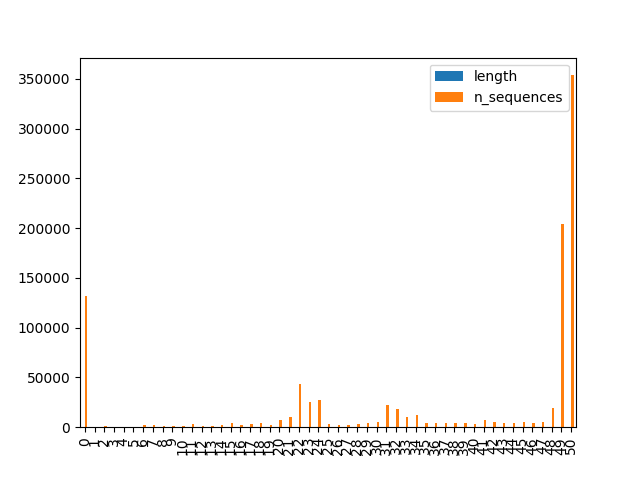
\includegraphics[width=11cm, height=7cm]{images/length-distr.png}
    \caption{Length distribution of the sequences after removing the adapter fragments}
    \label{length-distr}
\end{figure}

\newpage

\section{Task 2} \label{task2}

\paragraph{} The second task consists on developing an algorithm that identifies all the sequences in S that contain suffixes that match a prefix of a and where this suffix can contain up to a given percentage of mismatches to the prefix of the given adapter sequence.

\subsection{Imperfect suffix-prefix match} \label{imperfect}

\begin{lstlisting}[language=c++, caption=Recursive algorithm for imperfect suffix-prefix match]
int longestImperfectMatch(string s,
                          int longest,
                          int length,
                          int errors,
                          Node* node) {
    if (errors > maxTotalErrors) return longest;

    int maxErrors = length * (percentage / 100.0);
    if (s == "") {
        if (node->isWordEnd and errors <= maxErrors) 
            longest = max(length, longest);
        return longest;
    }

    int index = nuclToInt(s[0]);
    string nextStr = s[1:];

    if (node->isWordEnd and errors <= maxErrors) 
        longest = max(length, longest);

    ++length;

    for (int i = 0; i < node->childs.size(); ++i) {
        Node* child = node->childs[i];
        if (child != NULL) {
            if (i == index) 
                longest = max(longest, longestImperfectMatch(nextStr,longest, length, errors, child));
            else 
                longest = max(longest, longestImperfectMatch(nextStr, longest, length, errors+1, child));
        }
    }
    return longest;
}
\end{lstlisting}

\paragraph{} The worst asymptotic running time of this algorithm is linear respect to the size of the trie since what the algorithm is essentially doing is a depth first search.
The practical running time that we got depends on the percentage of error since the algorithm quits the search when the number of errors is bigger than the total maximum of errors that the whole sequence can have.
We got 20s for the 10\% error and 59s for the 25\% error.

\subsection{Imperfect suffix-prefix match allowing insertions and deletions}

\paragraph{} The difference between this and the previous section is how the errors are computed, in the previous one only missmatches were allowed, now insertions and deletions are also allowed.
In order to compute the errors now, we used the edit dynamic proogramming distance algorithm that computes the minimum number of operations to transform one string to an otherone.

\begin{lstlisting}[language=c++, caption=Dynamic programming algorithm to calculate the edit distance between two strings]
int editDistance(string s, string a) {
    int m = s.length() + 1, n = a.length() + 1;
    int[][] dp = int[m][n];
    for (int i = 0; i < m; ++i) {
        for (int j = 0; j < n; ++j) {
            if (i == 0) dp[i][j] = j;
            else if (j == 0) dp[i][j] = i;
            else if (s[i-1] == a[j-1]) dp[i][j] = dp[i-1][j-1];
            else {
                dp[i][j] = 1 + min(dp[i][j - 1],
                                   dp[i - 1][j],   
                                   dp[i - 1][j - 1]);
            }
        }
    }
    return dp[m-1][n-1];
}
\end{lstlisting}

\paragraph{} The new search algorithm has a few changes respect to the one in \ref{imperfect}: the rror computation and the arguments of it, since now we also need the current prefix and the current suffix all the time.

\begin{lstlisting}[language=c++, caption=Dynamic programming algorithm to calculate the edit distance between two strings]
int longestImperfectMatchID(string s,
                                   string suf,
                                   string pref,
                                   int longest,
                                   int length,
                                   Node* node) {
    int errors = editDistance(suf, pref);
    if (errors > maxTotalErrors) return longest;
    ...
    string nextSuf = suf;
    nextSuf.push_back(s[0]);
    for (int i = 0; i < node->childs.size(); ++i) {
        Node* child = node->childs[i];
        if (child != nullptr) {
            string nextPref = pref;
            nextPref.push_back(intToNucl(i));
            ...
        }
    }
    return longest;
}
\end{lstlisting}

\subsection{Results}

\begin{table}[H]
    \centering
    \begin{tabular}{| c | c | c |}
        \hline
        Error & Matches & 100\% match \\
        \hline
        \hline
        0\% & 646368 & 132149 \\
        10\% & 670925 & 141997 \\
        25\% & 708900 & 142569 \\
        10\% ID & 676781 & 147408 \\
        25\% ID & 713464 & 150729 \\
        \hline
    \end{tabular}
    \caption{Matches obtained allowing errors}
\end{table}

\begin{figure}[H]
    \centering
    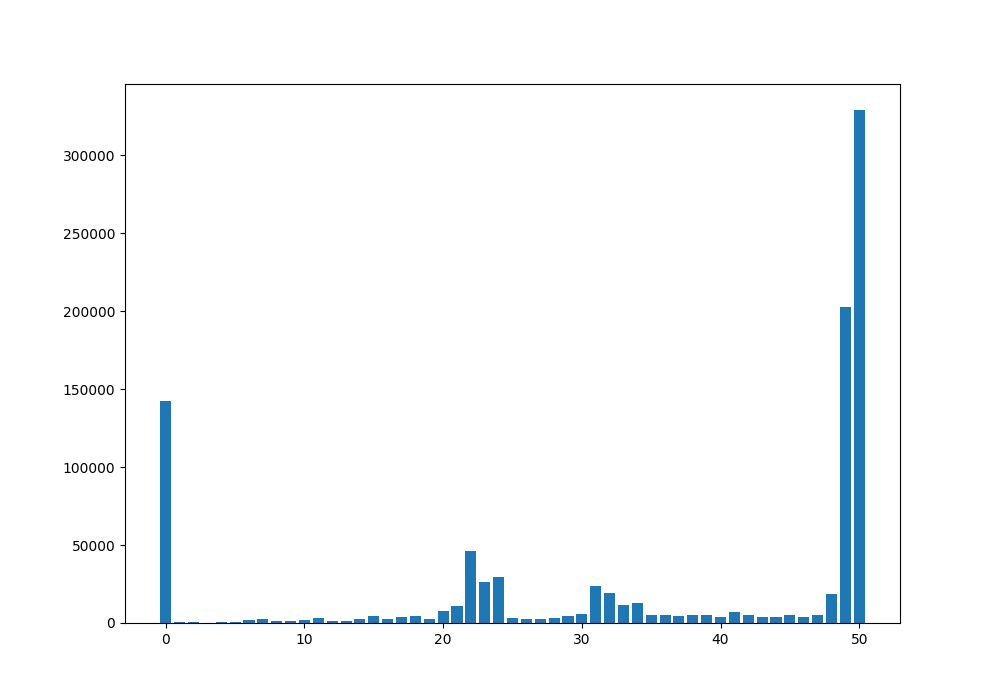
\includegraphics[width=11cm, height=7cm]{images/length-distr-10.png}
    \caption{Length distribution of the sequences after removing the adapter fragments with a 10\% of error}
    \label{length-distr-10}
\end{figure}

\begin{figure}[H]
    \centering
    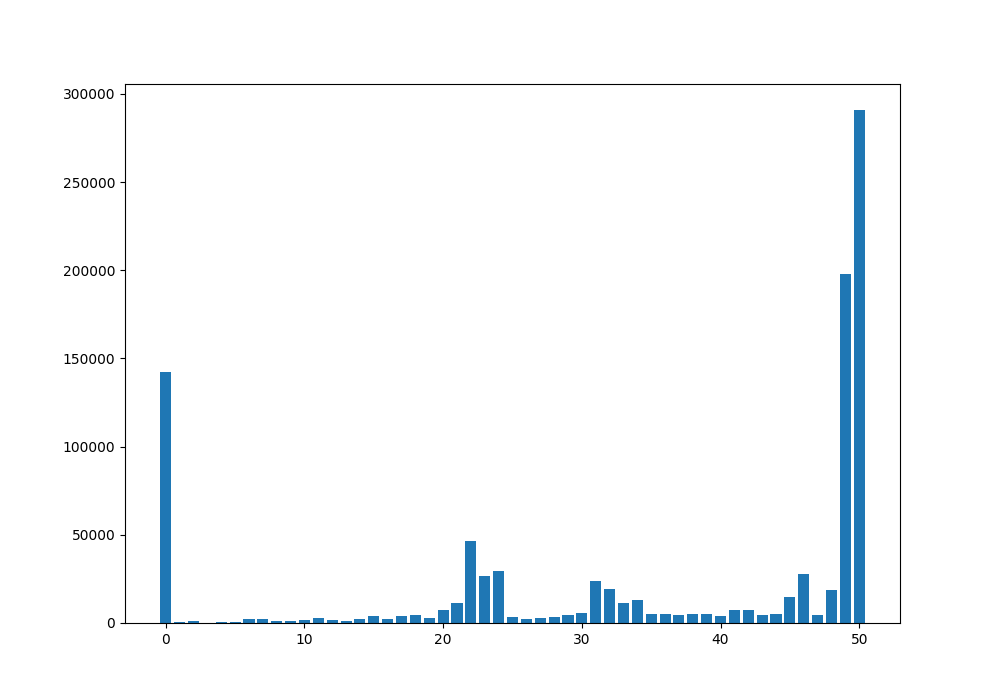
\includegraphics[width=11cm, height=7cm]{images/length-distr-25.png}
    \caption{Length distribution of the sequences after removing the adapter fragments with a 25\% of error}
    \label{length-distr-25}
\end{figure}

\begin{figure}[H]
    \centering
    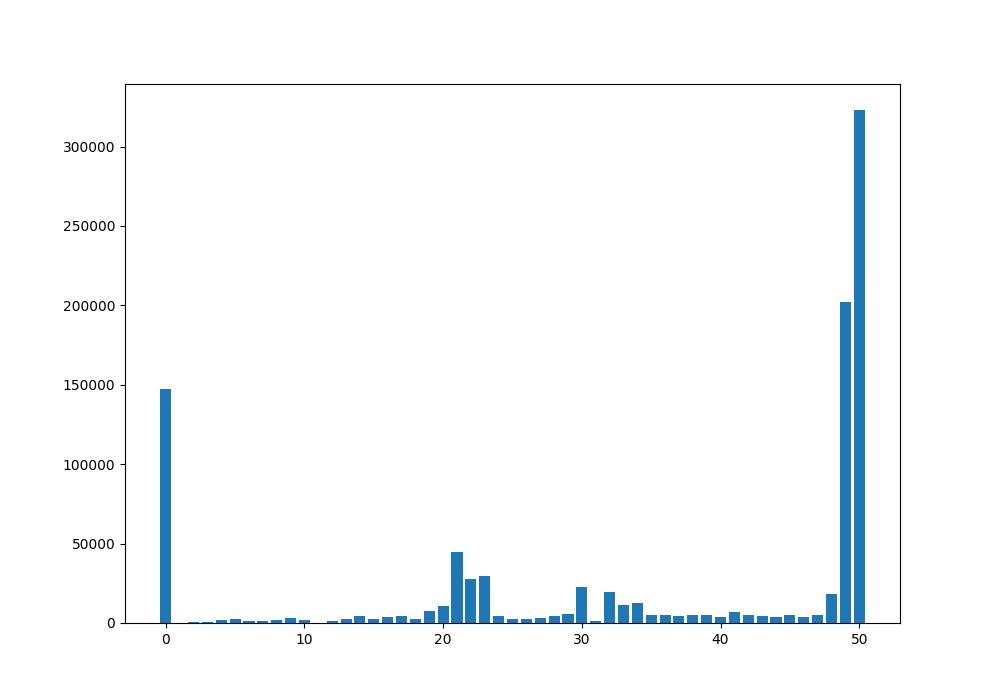
\includegraphics[width=11cm, height=7cm]{images/length-distr-10-id.png}
    \caption{Length distribution of the sequences after removing the adapter fragments with a 10\% of error allowing insertions and deletions}
    \label{length-distr-10-id}
\end{figure}

\begin{figure}[H]
    \centering
    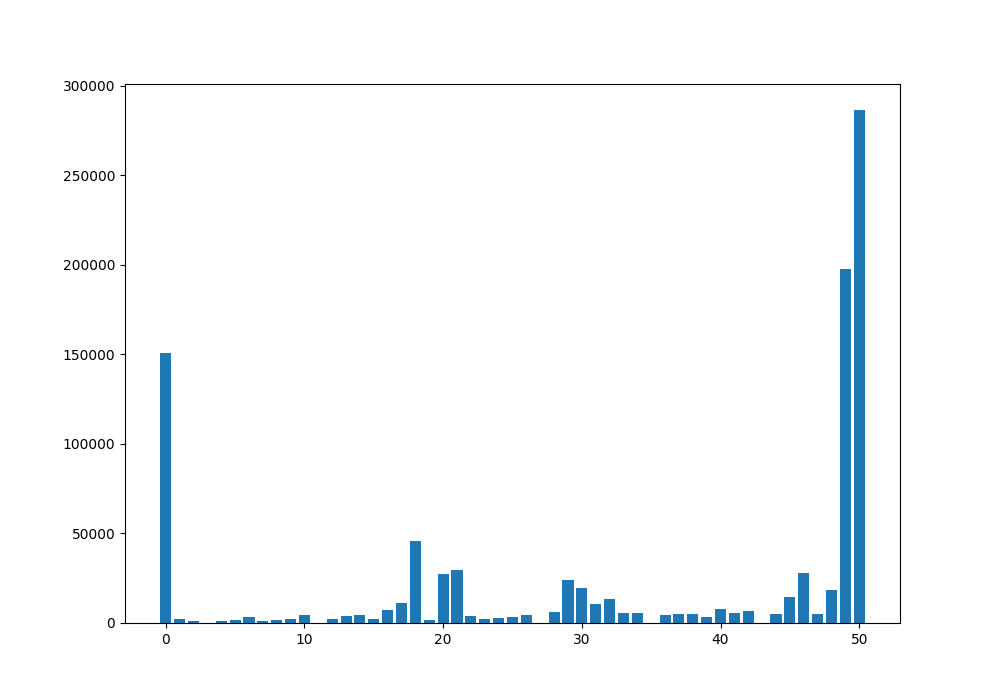
\includegraphics[width=11cm, height=7cm]{images/length-distr-25-id.png}
    \caption{Length distribution of the sequences after removing the adapter fragments with a 25\% of error allowing insertions and deletions}
    \label{length-distr-25-id}
\end{figure}

\newpage

\section{Task 3}

\newpage

\section{Task 4}

\newpage

\section{Task 5}

\newpage

\listoffigures

\listoftables

\end{document}
